\chapter{The 3-2-1 Speaking Trick That Forces You To Stop Rambling!}

This lecture is built around a small but useful algorithm for speaking under pressure. We begin, not with the framework itself, but with the failure mode that necessitates it: the mind branches too quickly, speech starts before structure has formed, and rambling replaces clear points. From there Zhang turns to a single scaffold, \((3,2,1)\), shows how it compresses the search space of thought, and then verifies its usefulness first on his own example and finally in a live pressure drill.

\section{Why We Ramble Under Pressure}

The opening move is diagnostic. Zhang does not yet tell us what to say; he asks what happens when a question arrives and we are not prepared. The answer is psychological but also structural: thought explodes into too many directions at once, and speech begins before an ordering principle is in place. The lecture’s first mathematical skeleton may therefore be written as
\begin{equation}
\text{unprepared question}
\;\Rightarrow\;
\text{panic search}
\;\Rightarrow\;
\text{rambling}.
\end{equation}
This is the initial causal chain. It explains why the experience is frustrating, embarrassing, and confidence-destroying. The important thing is that the problem is not merely lack of courage. It is lack of structure.

\subsection{Question \& Answer}

\paragraph{Question.} Why do we ramble when we are put on the spot?

\paragraph{Answer.} Because the mind begins searching before it has selected an organizing line. Zhang’s image of ``a dozen browser tabs'' is a vivid description of combinatorial explosion: many possible directions appear at once, none is privileged, and verbalization starts in the middle of that search. The result is not silence in the first instance, but disorder.

There is a second point in the opening that matters for the later notes. Zhang inserts personal testimony before he introduces the solution. He used to do this; he knows the feeling. That move gives the framework motivational weight. We are not merely receiving a trick. We are receiving a response to a genuine recurrent failure.

\section{From Rambling to Frameworks}

The next pivot is from diagnosis to fallback. Zhang contrasts prepared and unprepared speaking. Prepared content feels more confident; off-the-cuff speaking feels less confident. The lecture then sharpens the issue with a direct question: if someone asks us something and we are not prepared, what do we fall back on?

The first answer is blunt: generally, rambling. Only after that answer does he introduce the replacement:
\begin{equation}
\text{no framework}
\;\Rightarrow\;
\text{fallback to rambling},
\qquad
\text{framework}
\;\Rightarrow\;
\text{fallback to structure}.
\end{equation}
This is the key transition of the lecture. Frameworks are not presented as ornamental presentation devices. They are fallback mechanisms. When spontaneity is required, we need something simple enough to reach for instantly.

Zhang then asks the room how many people already use frameworks when they communicate. The point of this audience check is to create a small gap: frameworks exist, they are useful, and yet most people do not consciously use them. Into that gap he inserts the lecture’s main object.

\section{The \texorpdfstring{$3,2,1$}{3,2,1} Framework}

The central object is introduced by name first, then by repetition, and only then by use. This order should remain visible in the chapter. We see the board title before the scaffold is fully operational.

\begin{figure}[h]
\centering

\includegraphics[width=0.72\textwidth]{lecture_13_figure_01.png}
\caption{Opening board: the lecture introduces \((3,2,1)\) explicitly as a framework.}
\end{figure}

The visible board content is minimal but important:
\begin{align}
\left(3,2,1\right), \qquad \left[\text{Framework}\right].
\end{align}
That is, the lecture first names the object before it defines it. Only afterwards do we get the operational expansion
\begin{align}
3 &\mapsto \text{steps},\\
2 &\mapsto \text{types},\\
1 &\mapsto \text{thing}.
\end{align}

\begin{figure}[h]
\centering
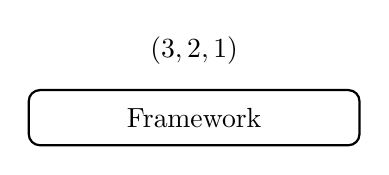
\begin{tikzpicture}[x=1cm,y=1cm]
\node at (0,1.4) {$\left(3,2,1\right)$};
\draw[thick,rounded corners] (-2.1,0.2) rectangle (2.1,0.9);
\node at (0,0.55) {Framework};
\end{tikzpicture}
\caption{Minimal reconstruction of the opening board label.}
\end{figure}

\begin{definition}
For a topic \(T\), we write the lecture’s scaffold editorially as
\begin{equation}
F_{321}(T)
=
\bigl(
\text{3 steps for }T,\;
\text{2 types of }T,\;
\text{1 thing about }T
\bigr).
\end{equation}
This is note-writing notation, not lecturer-written notation. Its purpose is to make explicit that the framework maps an open-ended topic into a small finite repertoire of answer shapes.
\end{definition}

\begin{remark}
Operationally, Zhang does not require us to begin from the first slot. His real pedagogical claim is more flexible:
\begin{equation}
\text{entry}(F_{321}(T))
\in
\left\{
\text{1 thing about }T,\;
\text{2 types/ways of }T,\;
\text{3 steps for }T
\right\}.
\end{equation}
We may begin where the mind can most easily get traction.
\end{remark}

\subsection{Question \& Answer}

\paragraph{Question.} What exactly does \(3,2,1\) mean?

\paragraph{Answer.} In its literal lecture form it means ``three steps, two types, one thing.'' But the deeper point is that it is a controlled repertoire of decompositions. We are not being told a single sentence to memorize. We are being handed three small answer-generating molds. This is why Zhang can say that he uses the same framework for social media content, for Q\&A, and when he has very little time to prepare.

Having defined the object, the lecture immediately moves to demonstration. That is essential. The framework is not left in symbolic form for long. It is tested on a random topic.

\section{Worked Example: Avocado}

Zhang asks the room for a topic and receives ``avocado.'' He then makes a pedagogically decisive choice: he starts with the easiest slot, the one thing. That is the local algorithm we should preserve in the notes. The framework reduces the search space by allowing entry through the simplest stable handle.

The left board in the workshop clip displays the scaffold clearly; the right board shows that this scaffold sits beside a broader staged framework.

\begin{figure}[h]
\centering

\includegraphics[width=0.82\textwidth]{lecture_13_figure_03.png}
\caption{Workshop boards: the left board gives the \(3,2,1\) scaffold, while the right board shows a separate staged framework.}
\end{figure}

The left board gives us the clean visible structure
\begin{equation}
3\ \text{steps},\ 2\ \text{types},\ 1\ \text{thing}.
\end{equation}
The right board is only partly legible, but it clearly presents a second staged framework with four levels:
\begin{equation}
S_1 \to S_2 \to S_3 \to S_4.
\end{equation}
We retain only that conservative structure, because the longer labels are not secure.

\begin{figure}[h]
\centering
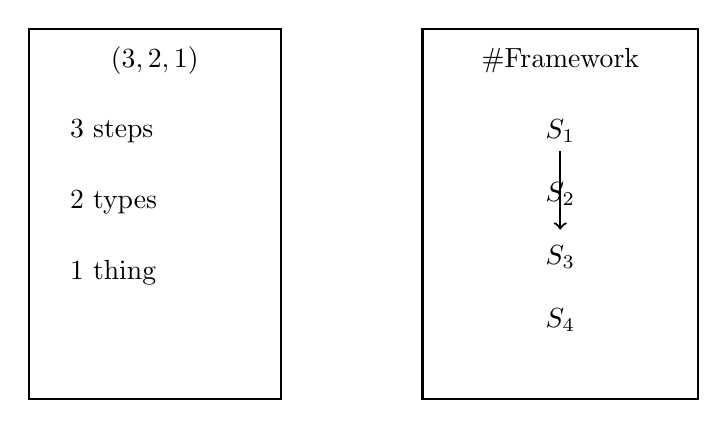
\begin{tikzpicture}[x=1cm,y=1cm]
\draw[thick] (-4.9,-0.2) rectangle (-1.7,4.5);
\node at (-3.3,4.1) {$\left(3,2,1\right)$};
\node[anchor=west] at (-4.5,3.2) {$3$ steps};
\node[anchor=west] at (-4.5,2.3) {$2$ types};
\node[anchor=west] at (-4.5,1.4) {$1$ thing};

\draw[thick] (0.1,-0.2) rectangle (3.6,4.5);
\node at (1.85,4.1) {\#Framework};
\node at (1.85,3.2) {$S_1$};
\node at (1.85,2.4) {$S_2$};
\node at (1.85,1.6) {$S_3$};
\node at (1.85,0.8) {$S_4$};
\draw[->,thick] (1.85,2.95) -- (1.85,1.95);
\end{tikzpicture}
\caption{Clean reconstruction of the visible workshop board structure.}
\end{figure}

We can now record the avocado example in the lecture’s own spirit. In lecture order the scaffold is
\begin{equation}
F_{321}(\text{avocado})
=
\bigl(
\text{3 preparation steps},
\text{2 ways to have it},
\text{1 thing about it}
\bigr),
\end{equation}
but in performance Zhang enters through the last component because it is easiest.

The derivation of the example proceeds as follows.
\begin{enumerate}
\item Choose the topic \(T=\text{avocado}\).
\item Select the easiest entry point: one thing.
\item Produce a single salient claim: avocado is excellent on a keto diet.
\item Expand to two ways: on toast, or eaten like a fruit.
\item Expand to three steps: cut it, mash it, season it.
\end{enumerate}
This is not a proof of a proposition. It is a controlled reduction of an open-ended search problem.

\subsection{Question \& Answer}

\paragraph{Question.} How does the framework give the brain something to lean on?

\paragraph{Answer.} By suppressing uncontrolled branching. Zhang dramatizes the alternative: once we begin without a framework, the mind ricochets through color, ripeness, storage, recipes, and other irrelevant branches. In editorial shorthand,
\begin{equation}
\text{avocado}
\;\Rightarrow\;
\{\text{green},\text{ripe},\text{storage},\text{recipes},\ldots\}
\;\Rightarrow\;
\text{blankness}.
\end{equation}
The framework works by replacing this uncontrolled branching with a finite menu of admissible moves.

The lecture then makes a further important point. The same scaffold accommodates different kinds of structure. It is not limited to description. ``Two types'' can become ``two ways,'' and ``three steps'' gives a procedural decomposition. The framework is therefore both classificatory and procedural.

\section{Pressure, Pause, and a Larger Toolkit}

After the avocado example, Zhang turns to the viewer and anticipates the next objection: all right, but can I do this? That is the natural next question, and it is answered not by theory but by a live drill. Before the drill concludes, however, the lecture pauses for a brief aside: \(3,2,1\) is only one of several communication frameworks.

That brief aside is visually supported by the inserted board shot.

\begin{figure}[h]
\centering

\includegraphics[width=0.78\textwidth]{lecture_13_figure_04.png}
\caption{Inserted board shot: \(3,2,1\) appears as one item inside a broader framework hierarchy.}
\end{figure}

What matters in this frame is not the promotional banner at the bottom, which we ignore, but the board hierarchy at the top:
\begin{equation}
\text{Visibility},
\qquad
2)\ \left(3,2,1\right).
\end{equation}
The lecture is briefly placing the scaffold inside a wider inventory of frameworks rather than replacing it with new mathematics.

\begin{figure}[h]
\centering
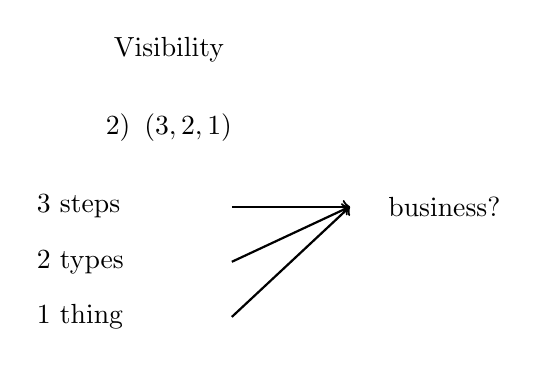
\begin{tikzpicture}[x=1cm,y=1cm]
\node at (0,3.9) {Visibility};
\node at (0,2.9) {$2)\ \left(3,2,1\right)$};

\node[anchor=west] at (-1.8,1.9) {$3$ steps};
\node[anchor=west] at (-1.8,1.2) {$2$ types};
\node[anchor=west] at (-1.8,0.5) {$1$ thing};

\draw[->,thick] (0.8,1.9) -- (2.3,1.9);
\draw[->,thick] (0.8,1.2) -- (2.3,1.9);
\draw[->,thick] (0.8,0.5) -- (2.3,1.9);
\node at (3.5,1.9) {business?};
\end{tikzpicture}
\caption{Conservative reconstruction of the visible board hierarchy and connector lines.}
\end{figure}

\subsection{Question \& Answer}

\paragraph{Question.} Can we actually use this under pressure, or is it only convincing in the lecturer’s own example?

\paragraph{Answer.} The lecture’s answer is that we can, provided we do not burden ourselves with using all three slots at once. Zhang explicitly says that the student may pick whichever slot is easiest. This is the operational point:
\begin{equation}
\text{pick one admissible slot first}
\;\Rightarrow\;
\text{stabilize the answer}
\;\Rightarrow\;
\text{expand only if needed}.
\end{equation}
The framework is not a performance burden. It is a relief mechanism.

The three-second countdown that follows is therefore not theatrical decoration. It is a stress test. The lecture is now ready to close the original problem it posed at the start.

\section{Live Drill: Travel and the Psychology of Readiness}

The random topic now becomes ``travel,'' and the student executes the scaffold quickly. The lecture resolves its own tension by moving through the same three slots on a new topic and showing that the transfer works.

In lecture order we may summarize the successful response as
\begin{equation}
F_{321}(\text{travel})
=
\bigl(
\text{plan, book, go},
\text{regional/international},
\text{magnificent}
\bigr).
\end{equation}
The student’s actual performance begins with the one thing, then moves to two types, then to three steps. That order matters, because it confirms the practical flexibility emphasized earlier.

The demonstration now yields a final interpretation. Zhang does not stop at saying the answer was correct. He draws a psychological conclusion. The student leaned into the microphone, moved forward, and appeared ready. Preparedness here is not merely cognitive. It is embodied. That is why the lecture’s closing equation is not really about content at all:
\begin{equation}
\text{framework}
\;\Rightarrow\;
\text{readiness}
\;\Rightarrow\;
\text{confident communication}.
\end{equation}

\subsection{Question \& Answer}

\paragraph{Question.} Why does a framework change not only what we say, but how ready we feel?

\paragraph{Answer.} Because once the mind knows that a stable answer shape is available, speaking ceases to feel like an uncontrolled fall. The framework does not merely fill the mouth with words; it gives the body permission to move toward the task instead of away from it. That is why Zhang contrasts excitement with fear at the end. When we are unprepared, we do not want to communicate. When we have a framework, we lean into communication.

\section{Summary}

The lecture’s structure is remarkably tight. We begin with a failure mode: an unprepared question produces panic search and rambling. We then identify the missing object, namely a framework to fall back on. The lecture introduces \((3,2,1)\), defines it as three steps, two types, one thing, and immediately shows that it reduces the search space of thought.

The avocado example provides the worked mechanism; the travel example provides the proof of transfer. The brief aside about other frameworks broadens the frame without changing the central lesson. What remains at the end is a small speaking algorithm: reduce an open topic to one of a few admissible shapes, begin from the easiest slot, and let structure replace panic. That is the mathematical payload of the talk, and it is why such a simple mnemonic can carry so much practical force.